
\begin{frame}[label=exp]{Experimentation}
	\textbf{And then}
	
	\begin{itemize}
	\item Evaluate the accuracy of the prediction algorithm.
	\item Replicate the calling process, by:
		\begin{itemize}
			\item Holding back one data point
			\item Training the system with $N-1$ data points
			\item Predicting the holded back data Point Occupancy Code
			\item Cycling through all data points, to get average prediction accuracy
		\end{itemize}
	\item Use accuracy evaluation to compare
		\begin{itemize}
			\item a dummy classifier and traditional NLP elements
			\item Traditional NLP metrics and the improvements from this project's work
		\end{itemize}
	\end{itemize}
	
\end{frame}

\begin{frame}[label=exp]{Experimentation}
	\textbf{Data Source Used}
	
	\begin{itemize}
		\item Data from Yellow Pages
		\item Graduately gather over a 10 day period
		\item Counting 1593 data points
	\end{itemize}
	
\end{frame}



\begin{frame}[label=exp]{Experimentation}
	\textbf{the Dummy Classifier Performance}
	
	\begin{itemize}
		\item Define the dummy classifier 
		\begin{itemize}
			\item Classifier that would always select the class
		\end{itemize}
		
	\end{itemize}
	
\end{frame}

\begin{frame}[label=exp]{Experimentation}
	
	\begin{figure}
		\caption{Dummy Classifier vs Traditionnal NLP}
		\centering
		\makebox[\textwidth]{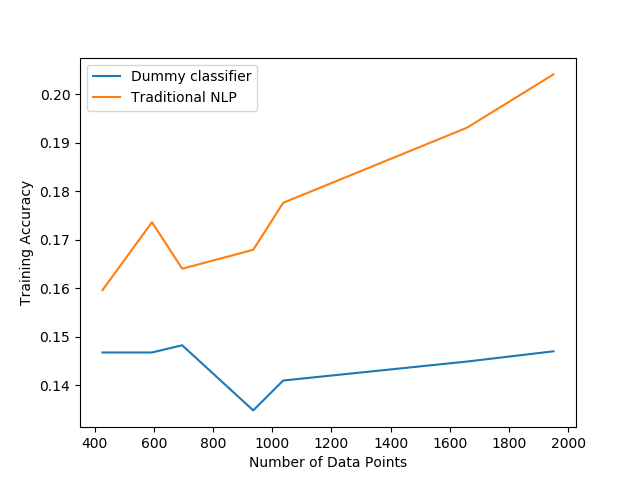
\includegraphics[width=0.7\textwidth, height=0.7\textheight]{images/dummy_vs_nlp.png}}
	\end{figure}
	
\end{frame}




\begin{frame}[label=exp]{Experimentation}
	\begin{figure}
		\caption{Dummy Classifier vs Traditionnal NLP}
		\centering
		\makebox[\textwidth]{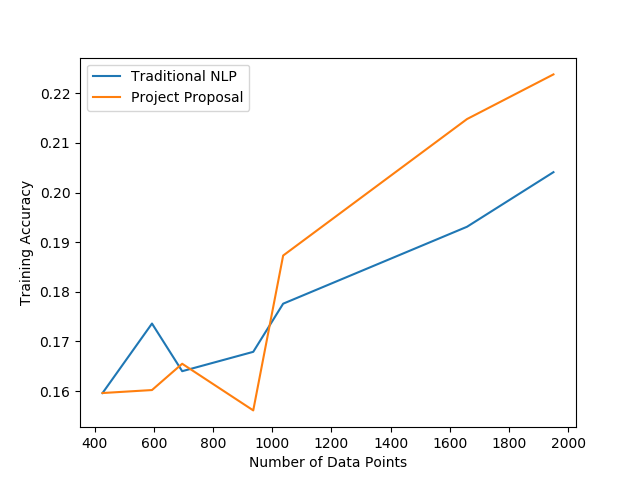
\includegraphics[width=0.7\textwidth, height=0.7\textheight]{images/nlp_vs_project.png}}
	\end{figure}
	
\end{frame}



